\chapter{Technical Background}
\label{capitulo3}

In this chapter an overview about the main concepts of this work will be described. The present section is divided in three major sections. In Section \ref{sensors}, the concepts of sensors is defined. In Section \ref{ml-ai}, the main concepts regarding machine learning and artificial intelligence are described. In Section \ref{autonomous-vehicles} is defined the major concepts about autonomous vehicles.

\section{Sensors}\label{sensors}

It is possible to have more sensors in autonomous vehicles, but these three sensors are the most common in autonomous vehicles structure. As is positioned in the Figure \ref{fig:autonomous-vehicles} the correct place for the most important sensors.


\begin{figure}[H]
\centering
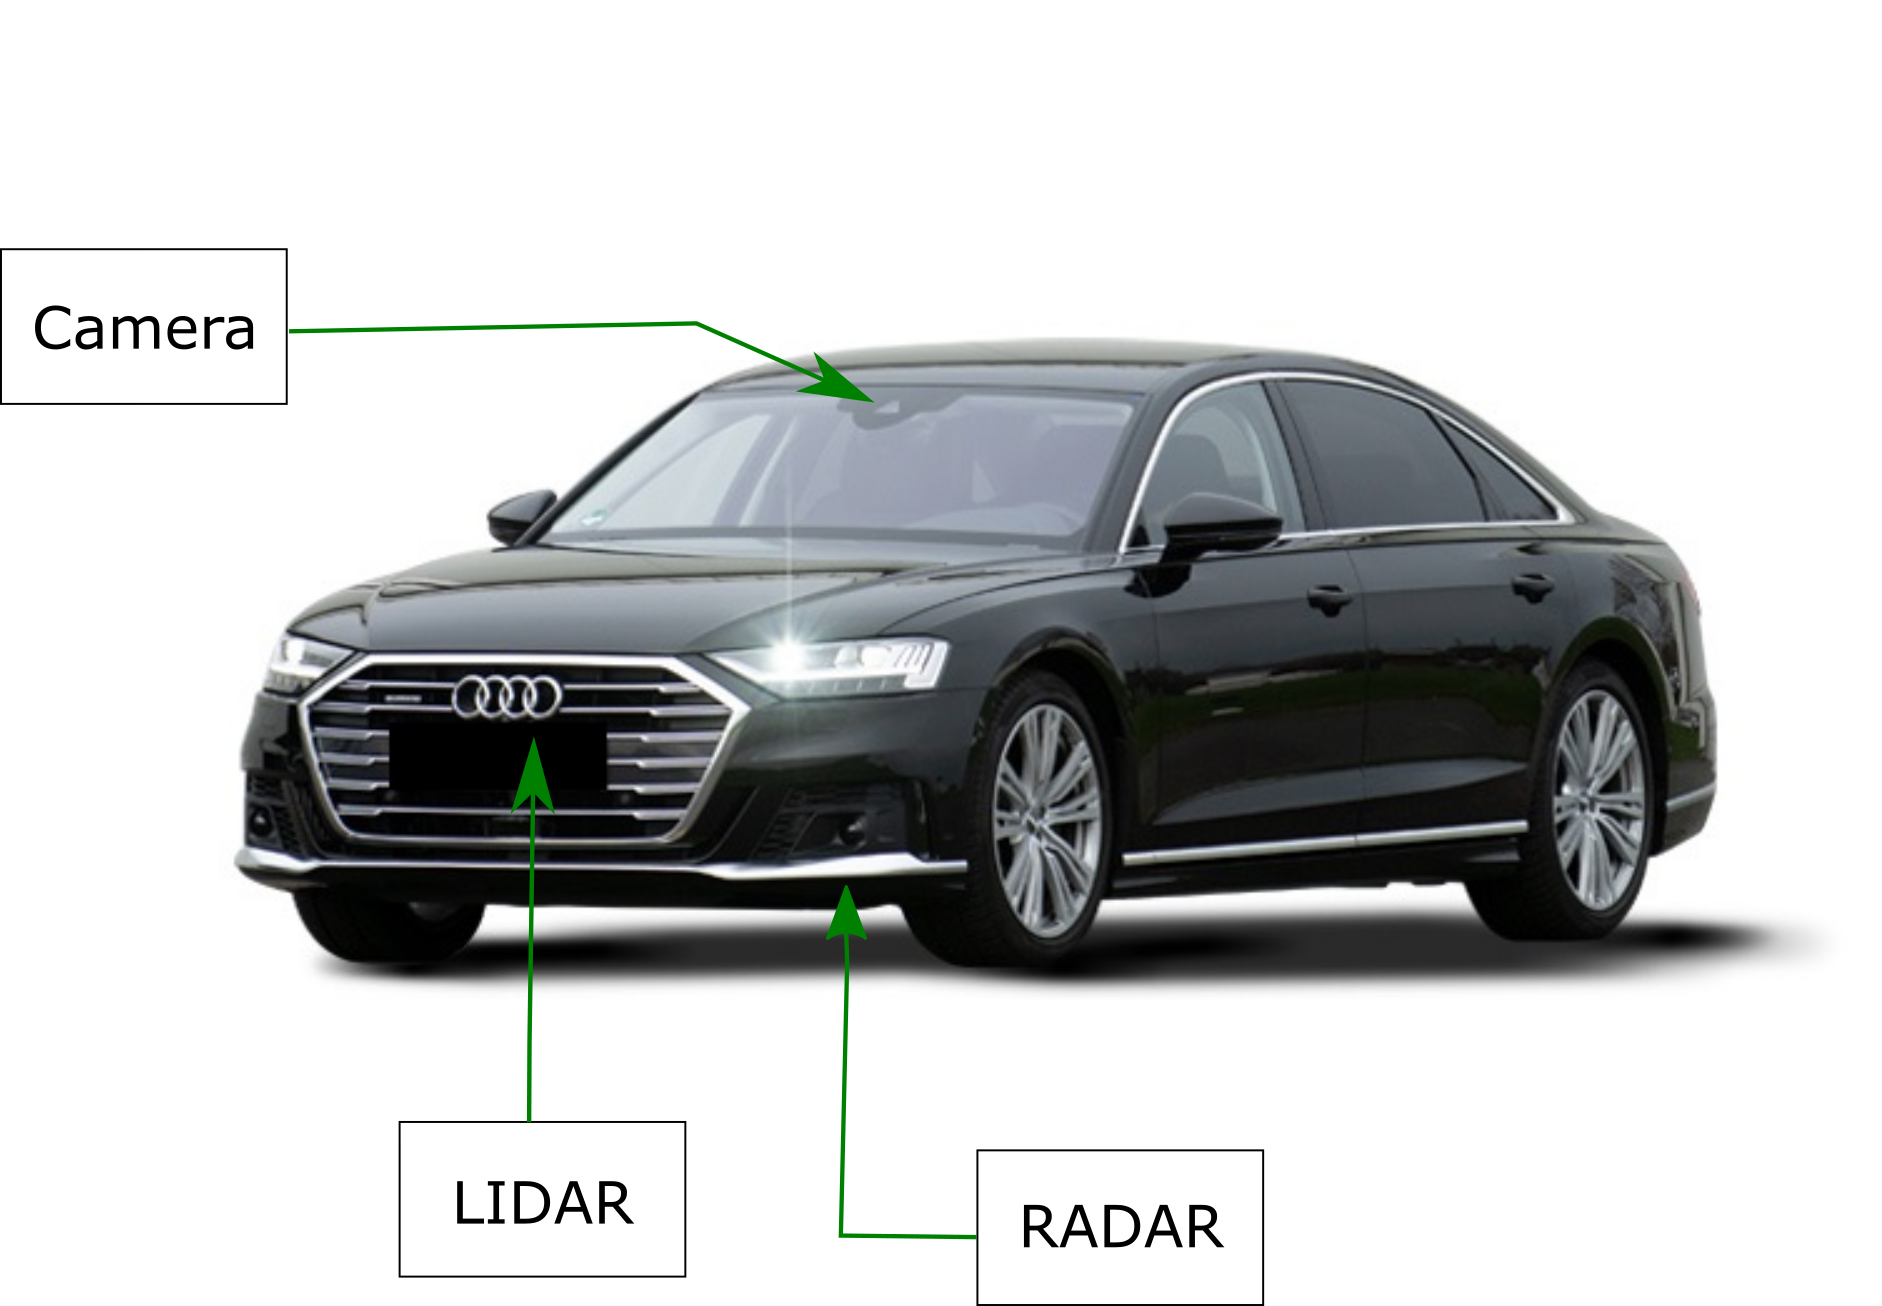
\includegraphics[scale=0.7]{imagens/image823.png}
\caption{Representation of an autonomous vehicle}
\label{fig:autonomous-vehicles}
\end{figure}


\subsection{Camera}
The camera is a kind of sensor whose allows the car to see the environment using the collected image, in Figure \ref{fig:camera} is shown the standard camera for autonomous vehicles.

It is an optical instrument for image or video capture of images in the same size, for example, there are some cameras where it is possible to set up the numbers of frames per second (FPS) and the image resolution. 

Also, it is important to remember the importance of the calibration of the cameras, the Equations for this process were available in \cite{888718}. This step is very important to acquire the real size of the objects, because sometimes is necessary to compare the size of these objects. 

\begin{figure}[H]
\centering
\includegraphics[width=\columnwidth]{imagens/camera.png}
\caption{Representation of a camera of the autonomous vehicle}
\label{fig:camera}
\end{figure}

This sensor allows the car to detect a lot of objects and at the same time it is possible to perform object recognition as well. It is necessary to freeze the difference between object detection and object recognition. There are different algorithms to perform these tasks. The proposed algorithm in Chapter \ref{capitulo4} performs the both detection combined with the distances estimation. 

\subsection{Radar}

The automotive radio detection and ranging (RADAR) sensors has the responsibility to perform object detection around the vehicle and avoid a potential collisions. With this sensor is possible to warn the driver and combined with level 1 of automation as already shown in Figure \ref{fig:automation} to intervene with the brake the car or use other controls to prevent an accident \cite{ariyur2006collision}.

\begin{figure}[H]
\centering
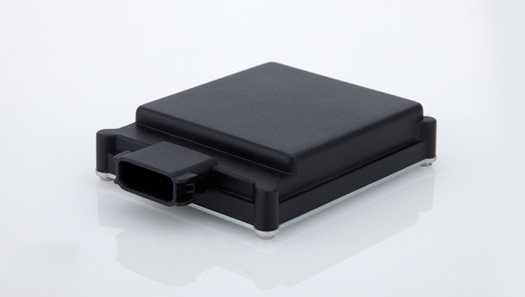
\includegraphics[width=\columnwidth]{imagens/radar.jpg}
\caption{A commercial radar model ARS430 CV from Continental}
\label{fig:camera}
\end{figure}

Another interesting application of the RADAR in the automotive scenario is the capability to measure the relative speed to the vehicle and other objects, with that it is possible to estimate correctly the distance \cite{stevenson2011long}.

It is possible to combine the camera and RADAR and get a new kind of sensor as defined in \cite{kamerad}. With this approach is possible to react 160 times faster than a human driver.

\subsection{Lidar}
In Figure \ref{fig:lidar} is shown a light detection and ranging (LIDAR). The main purpose of this laser is to detect and track any kind of objects. 
\begin{figure}[H]
\centering
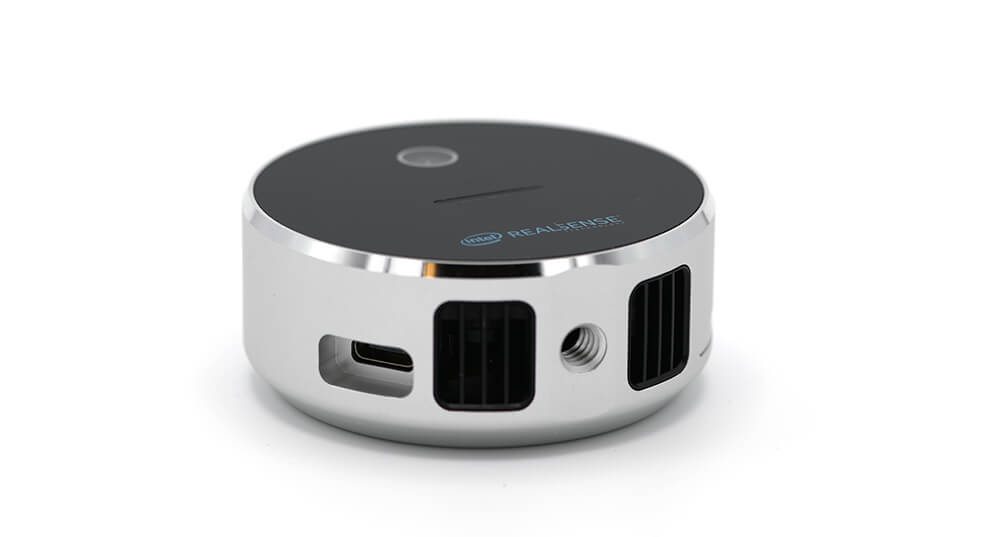
\includegraphics[width=\columnwidth]{imagens/lidar.jpg}
\caption{An exemple of a lidar of the autonomous vehicle}
\label{fig:lidar}
\end{figure}

This measurement is based on many times rotate this sensor in different directions, to scan the whole area of the autonomous vehicles is driving and collect some data for detect the objects \cite{gao2018object}.

\section{Machine Learning}\label{ml-ai}
The machine learning is approach based on algorithms to create some predictions, these techniques are based on mathematical and computer science, it is possible to apply this in several fields of the science. 
\subsection{Artificial Neural Networks}

The artificial neural networks (ANN) or percpetron were inspired in the human brain. This approach is because the capacity of the human brain to categorize new information. In Figure \ref{fig:ann} is shown an example of the structure of an ANN. Where there is an input array with the processed features for categorization. The next step of the processing is to define the weights for this analysis. The activation function is the main part of this process, because in this step the algorithm will transform the numbers collect by the previous steps and will return only in binary purpose, like $0$ and $1$ in the output layer \cite{goodfellow2016deep}.

\begin{figure}[H]
\centering
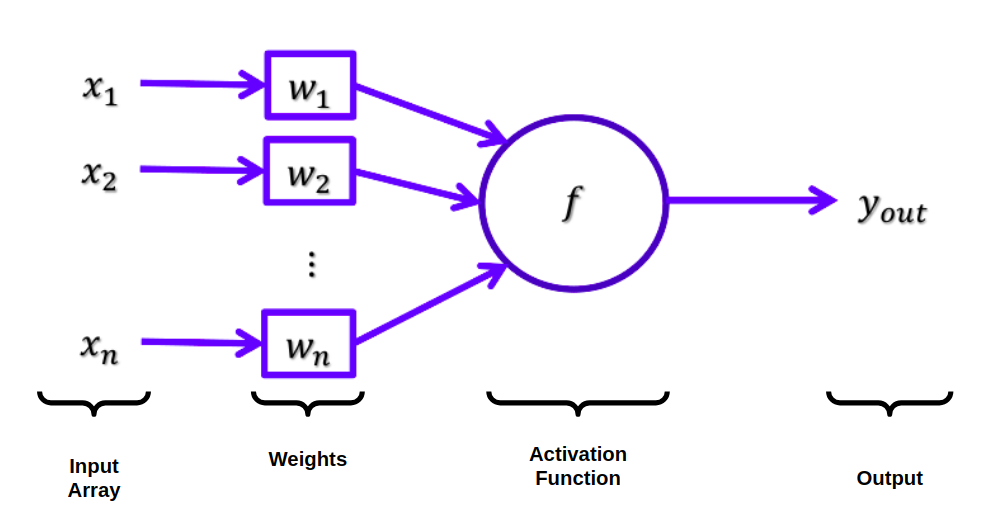
\includegraphics[width=\columnwidth]{imagens/ann.png}
\caption{The structure of an ANN}
\label{fig:ann}
\end{figure}

So, mathematically, the neuron output is a function of weighted sum of its inputs. Figure \ref{fig:ann_weight} is shown the mathematical background. Where $f$ is activation function, $w_i$ are the weights, and $\beta$ is the constant input called as bias.


\begin{figure}[H]
\centering
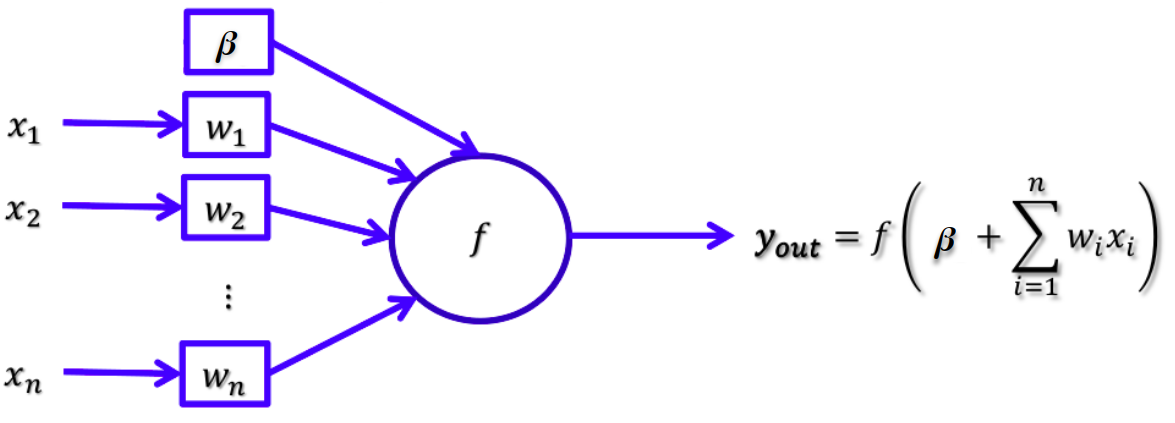
\includegraphics[width=\columnwidth]{imagens/math_ann_bias.png}
\caption{Mathematical representation of ANN with bias}
\label{fig:ann_weight}
\end{figure}


\subsubsection{Activation functions}
There are many different activation functions to use. These are crucial for the ANN characteristics, such as learning ability and computational efforts in terms of training and validation.

\begin{itemize}
    \item Unit step function
    \item Sign function
    \item Identity function
    \item Sigmoid function
    \item Hyperbolic tangent function
    \item Retified linear unit (Relu) 
\end{itemize}

\begin{table}[H]
\label{tab:tab1} 
\caption{Comparison Table for Activation Functions}
\centering
\resizebox{15.3cm}{!}{%
\begin{tabular}{|c|c|c|c|c|c|c|}
\hline
\textbf{\begin{tabular}[c]{@{}c@{}}Activation\\ Function\end{tabular}}  & \textbf{Linear}          & \textbf{Monotonic} & \textbf{Continuous}      & \textbf{\begin{tabular}[c]{@{}c@{}}Derivative \\ Monotonic\end{tabular}} & \textbf{\begin{tabular}[c]{@{}c@{}}Derivative\\ Continuous\end{tabular}} & \textbf{\begin{tabular}[c]{@{}c@{}}Simetric with \\ respect to \\ The Origin\end{tabular}} \\ \hline
{\color[HTML]{000000} Unit Step} & {\color[HTML]{FE0000} x} & {\color[HTML]{009901} \checkmark}& {\color[HTML]{FE0000} x} & {\color[HTML]{FE0000} x} & {\color[HTML]{FE0000} x} & {\color[HTML]{FE0000} x} \\ \hline
Sign & {\color[HTML]{FE0000} x} & {\color[HTML]{009901} \checkmark}& {\color[HTML]{FE0000} x} & {\color[HTML]{FE0000} x} & {\color[HTML]{FE0000} x} & {\color[HTML]{009901} \checkmark} \\ \hline
Identity & {\color[HTML]{009901} \checkmark}& {\color[HTML]{009901} \checkmark}& {\color[HTML]{009901} \checkmark}& {\color[HTML]{FE0000} x} & {\color[HTML]{009901} \checkmark}& {\color[HTML]{009901} \checkmark}\\ \hline
Sigmoid                                                                 & {\color[HTML]{FE0000} x} & {\color[HTML]{009901} \checkmark}             & {\color[HTML]{009901} \checkmark}                   & {\color[HTML]{FE0000} x}                                                 & {\color[HTML]{009901} \checkmark}                                                                   & {\color[HTML]{FE0000} x}                                                               \\ \hline
\begin{tabular}[c]{@{}c@{}}Hyperbolic\\ Tangent\end{tabular}            & {\color[HTML]{FE0000} x} & {\color[HTML]{009901} \checkmark}             & {\color[HTML]{009901} \checkmark}                   & {\color[HTML]{FE0000} x}                                                 & {\color[HTML]{009901} \checkmark}                                                                   & {\color[HTML]{009901} \checkmark}                                                                                 \\ \hline
\begin{tabular}[c]{@{}c@{}}Rectified \\ Linear Unit \\ (ReLU)\end{tabular} & {\color[HTML]{FE0000} x} & {\color[HTML]{009901} \checkmark}              & {\color[HTML]{009901} \checkmark}                   & {\color[HTML]{009901} \checkmark}                                                                   & \begin{tabular}[c]{@{}c@{}}{\color[HTML]{FE0000} x}\\ (at 0)\end{tabular}                       & {\color[HTML]{FE0000} x}                                                               \\ \hline
\end{tabular}}
\end{table}

In this work, Relu is the activation function chosen activation. Its mathematical definition is show in (\ref{eq:relu}). 


\begin{equation}
\label{eq:relu}
    f(x) = \mathrm{R}(x) = \mathrm{max}(0,x)
\end{equation}


The graphic visualization of the function Relu is shown in Figure \ref{fig:relu}, where this function return $0$ if the number from the weighted sum is below than $0$, or return $x$ if the previous value is over than $0$.


\begin{figure}[H]
\centering
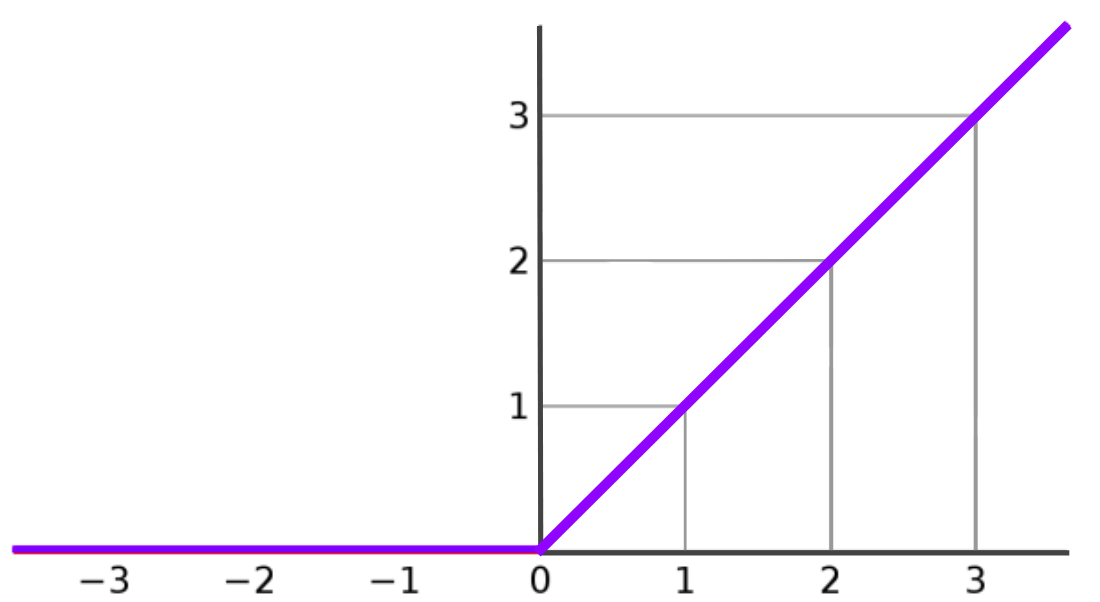
\includegraphics[scale=0.3]{imagens/relu_corrected.png}
\caption{The behavior of the Relu}
\label{fig:relu}
\end{figure} 

These are the important characteristics of this activation function.

    \begin{itemize}
        \item Widely used in deep networks
        \item Pros: nonlinear, monotonic, derivative monotonic, and fast convergence
        \item Cons: not continuously differentiable at zero, i.e. issues with gradient descent around origin.
    \end{itemize}

\subsubsection{Layered Neural Networks}

The quint essential example of a deep learning model is the multilayer perceptron (MLP). A MLP is just a mathematical function mapping some set of input values to output values. The function
is formed by composing many simpler functions \cite{goodfellow2016deep}.


These are the quint essential deep learning models. The goal
of a feedforward network is to approximate some function $f*$. For example, for a classifier, $y = f*(x)$ maps an input x to a category y. A feedforward network
defines a mapping $y = f (x; \theta)$ and learns the value of the parameters $\theta$ that resultin the best function approximation.

These models are called feedforward because information flows through the function being evaluated from $x$, through the intermediate computations used to define $f$, and finally to the output $y$. There are no feedback connections in which outputs of the model are fed back into itself.



\subsection{Convolutional Neural Networks}\label{sec:cnn}


The Convolutional Neural Networks (CNN) are a specialized kind of neural network for processing data that has a known \cite{lecun1995convolutional}. For example in autonomous vehicles domain, this approach is several used for object detection and object identification. This name  indicates that the network employs a mathematical operation called
convolution. 

A CNN coarsely scans the image for features (in lower dimension space), pools possible patterns, then inspect those patterns in detail with its fully connected
subnetworks, generating their classifications. In Figure \ref{fig:cnn_car} is defined the full process of this neural network. Where there are three other importants is steps: Convolutional layer is defined in Subsection \ref{sub:conv}. The pooling layer is introduced in the Subsection \ref{sub:pooling}.
\begin{figure}[H]
\centering
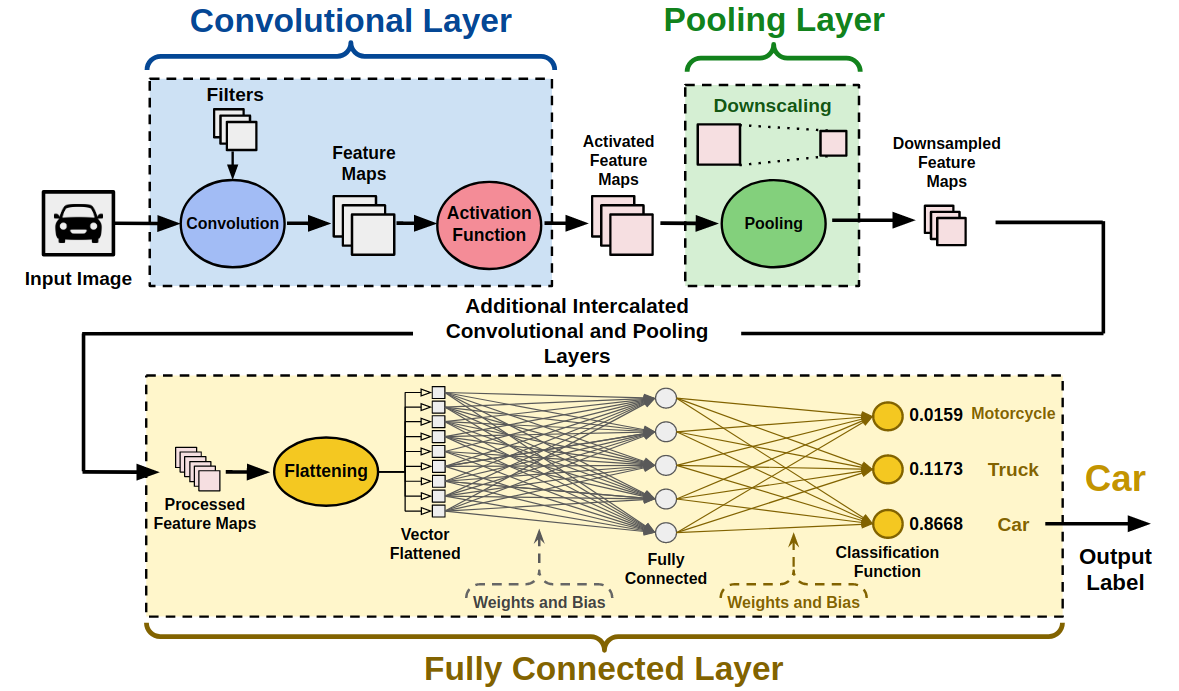
\includegraphics[width=\columnwidth]{imagens/Full_Process.png}
\caption{Full process of a convolutional neural network}
\label{fig:cnn_car}
\end{figure}


\subsubsection{Convolutional Layer}
\label{sub:conv}

When the convolutional layer is introduced, common inputs are tridimensional matrix with height and width defined accordingly with the image dimensions and determined by the amount of colors. In general the images use three color channels, Red-Green-Blue (RGB) as is shown in Figure \ref{fig:rgb}.

\begin{figure}[H]
\centering
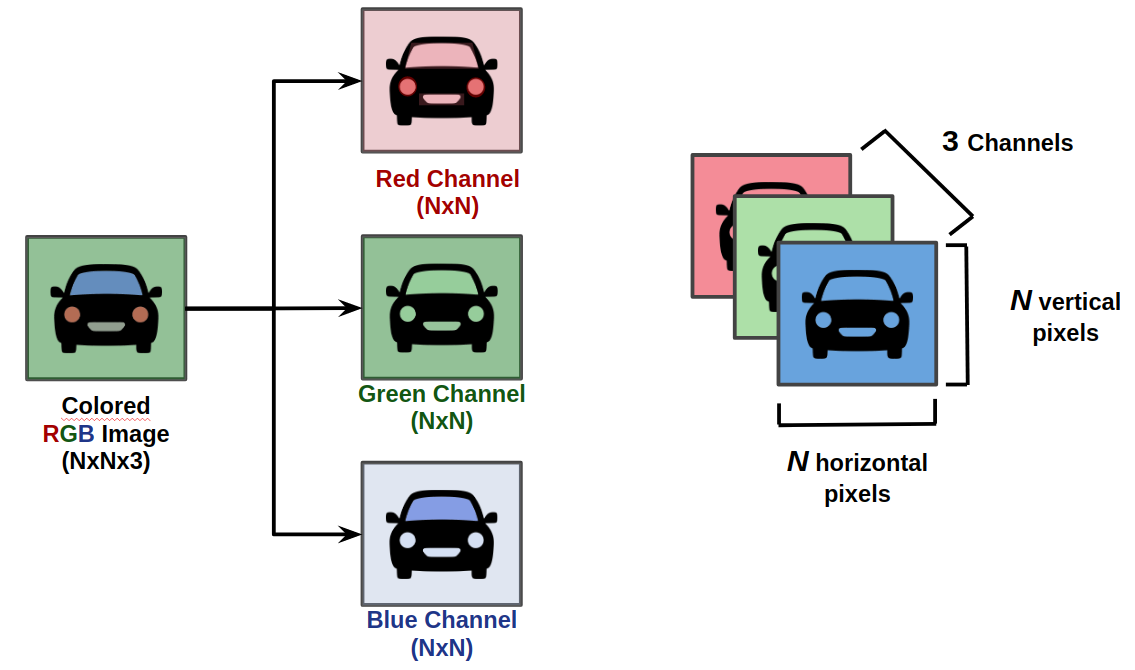
\includegraphics[scale=0.35]{imagens/rgb_representation.png}
\caption{Representation of the colors of the input image}
\label{fig:rgb}
\end{figure}


The convolutions work as filters that seem little squares and they are slipping through whole image and capturing the most important parts. For example in Figure \ref{fig:bias}, an image with $NxNX3$ and a filter with the $MxMX3$, where the main different is that each result is then summed, along with the Bias ($\beta$) value, to be then passed to the activation function. And in the end of the process generates a new matrix called as feature map or activation map.


\begin{figure}[H]
\centering
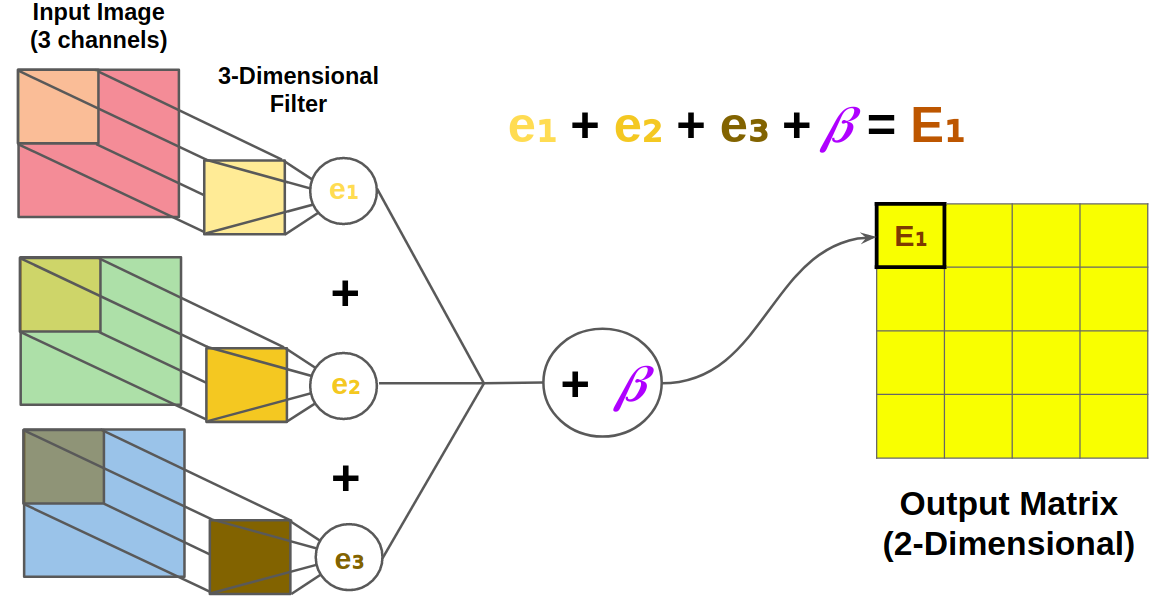
\includegraphics[scale=0.35]{imagens/three_dim_conv_2.png}
\caption{Representation of the convolution process}
\label{fig:bias}
\end{figure}




\subsubsection{Pooling and Upsampling}\label{sub:pooling}

A pooling layer is necessary to simplify the information from the previous layer. As happens with the convolution layer, it is choose an unit area, for example $2x2$ to slicing for the whole output information from the previous step. To brief, if the information from the previous layer was $4x4$, the output from process of pooling will be $2x2$. Nevertheless, the most used method is maxpooling, where the biggest number in the matrix is passed to the next step, this data summarization is used to reduce the amount of weights and to avoid overfitting. In Figure \ref{fig:pooling} is shown the maxpooling process.

\begin{figure}[H]
\centering
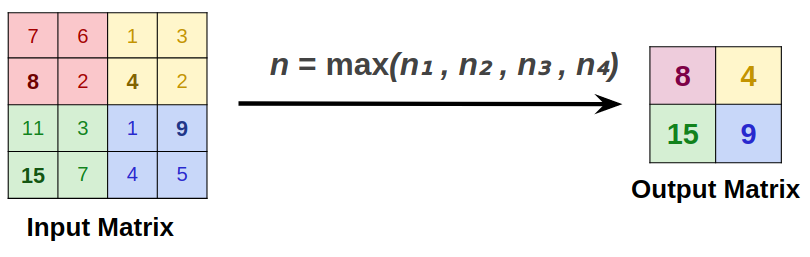
\includegraphics[scale=0.35]{imagens/max_pooling.png}
\caption{Representation of the maxpooling process}
\label{fig:pooling}
\end{figure}




\subsubsection{Auto-encoders}\label{auto-encoder}

It is a special type of neural network that is used to copy its inputs to its output. The intern structure is defined in Figure \ref{fig:autoencoder}. 

\begin{figure}[H]
\centering
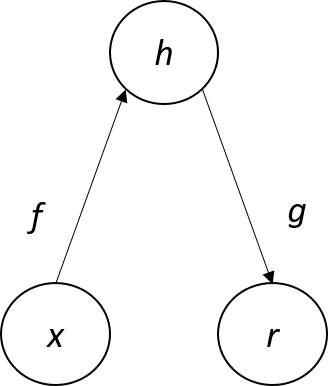
\includegraphics[scale=0.7]{imagens/autoencoder.png}
\caption{The structure of a standard autoenconder, where the variable $x$ means input and $r$ as an output through the internal representation in $h$. The encoder $f$ maps $x$ to $h$ and decoder $g$ maps $h$ to $r$}
\label{fig:autoencoder}
\end{figure}

As described in \cite{yang2020feedback}, this architecture has a hidden layer $h$ that describes a code used to represent the input. The network may be viewed as consisting of two parts: an encoder function $h=f(x)$ and a decoder that produces a reconstruction $r=g(h)$.

\subsubsection{Training}

In machine learning scenario, in special the neural networks domain epoch can be defined as a single forward pass and backward pass of all the training examples. It feeds in all the neurons into the network at once. Instead, it chooses a batch of neurons and feed them in. It performs stochastic gradient descent, and prevent our network from overfitting. There is difference between individual training step time and total training time \cite{pascanu2013difficulty}. 


\section{Autonomous Vehicles} \label{autonomous-vehicles}

In this section will be discussed the importance of the autonomous vehicles domain and its applicability on the society, and the problems occurred as well. 

\subsection{What are autonomous vehicles}
Modern vehicles now have Advanced Driver Assistance Systems (ADAS)
which work at several levels of autonomy, with these levels being
outlined by the National Highway Traffic Safety Administration
(NHTSA). The levels range from 0, no-automation, to 5, full selfdriving automation \cite{national2013preliminary}. An example of an ADAS is a parking system, proposed by \cite{krasner2016automatic}, that uses sensors to find the best way to maneuver a car into a parking space without driver input. Systems such as these are being used in modern semi-autonomous
vehicles as driver aids to hand over work from the driver to the
car’s systems \cite{schoning2006parklenkassistent}. As technology progresses, there will be a more
and more handover of control from the driver to the vehicle, level
4 of automation being the fully-autonomous state that is a prominent talking point in the automotive industry. The level 5 AV will
be able to self-drive anywhere (“full automation”), i.e. no cockpits,
drivers are not required to be fit to drive and even they do not require a driving license (every person in a vehicle is a passenger).

Actually, there are a lot of open datasets to allow new people to work with autonomous vehicles and hackthons as well. In the special the KITTI Dataset \cite{geiger2013vision} and NuScenes in \cite{caesar2020nuscenes}. These datasets provided data using GPS, Camera, RADAR and LIDAR. 

\subsection{Challenges}

The cities are not preparing for the autonomous vehicles at the same velocity of the industry. In the United States, for example, only of 6\% of the biggest cities from there are thinking or trying to create the necessary infrastructure to work with this new reality based on the data provided by \cite{cutler2015many}.

The process to put an autonomous vehicles on the street is very slow due to there a lot of other problems to take care such as the network even 3G, 4G or 5G, the conservation of the roads and the most important aspect is regarding the legislation. 

The study and development of this applications will change a lot of things in the society even at the sector of process until companies that work with delivery. But it is really necessary to control the traffic and reduce the accidents, follows the World Health Organization (WHO) every years over 1 million people lose their lives in car accidents and only in Brazil it is over than 47,000 deaths \cite{world2004world}. 
